\documentclass{lehramt-informatik-haupt}
\liLadePakete{mathe,syntaxbaum,automaten,formale-sprachen}
\usepackage{tikz}
\usetikzlibrary{shapes.geometric,calc}

\begin{document}

%%%%%%%%%%%%%%%%%%%%%%%%%%%%%%%%%%%%%%%%%%%%%%%%%%%%%%%%%%%%%%%%%%%%%%%%
% Theorie-Teil
%%%%%%%%%%%%%%%%%%%%%%%%%%%%%%%%%%%%%%%%%%%%%%%%%%%%%%%%%%%%%%%%%%%%%%%%

\chapter{Reguläre Sprachen}

\section{Chomsky-Hierarchie\footcite{wiki:chomsky}}

Im Jahr 1957 veröffentlichte der amerikanische Sprachwissenschaftler
Noam \memph{Chomsky} ein Regelwerk, mit dessen Hilfe sich formale
Grammatiken in \memph{vier Klassen} einteilen lassen:
\footcite[Seite 168]{hoffmann}

\begin{description}
\item[Typ 0] Phrasenstrukturgrammatik

Jede Grammatik ist per Definition immer auch eine Typ-0-Grammatik.
Insbesondere unterliegt die Struktur der Produktionen \memph{keinen
weiteren vereinbarten Einschränkungen}.

\item[Typ 1] kontextsensitive Grammatik

Eine Grammatik heißt kontextsensitiv, wenn jede Produktionsregel $l
\rightarrow r$ entweder die Beziehung \memph{$|r| \geq |l|$} erfüllt
oder die Form \memph{$S \rightarrow \epsilon$} aufweist. Ist die Regel
$S \rightarrow \epsilon$ enthalten, so darf $S$ in keiner anderen
rechten Seite einer Regel vorkommen.

\item[Typ 2] kontextfreie Grammatik

Typ-2-Grammatiken sind dadurch charakterisiert, dass die \memph{linke
Seite} einer Produktionsregel ausschließlich aus einer \memph{einzigen
Variablen} besteht. Für alle Produktionen $l \rightarrow r$ gilt also $l
\in V$.

\item[Typ 3] reguläre Grammatik\footcite[Seite 14]{theo:fs:1}

Reguläre Grammatiken sind kontextfrei und besitzen die zusätzliche
Eigenschaft, dass die rechte Seite einer Produktion entweder aus dem
\memph{leeren Wort $\epsilon$} oder einem \memph{Terminalsymbol},
\memph{gefolgt von einem Nonterminal}, besteht. Formal gesprochen
besitzt jede Produktion die Form $l \rightarrow r$ mit $l \in V$ und $r
\in \{ \epsilon \} \cup \Sigma V$ .
\end{description}

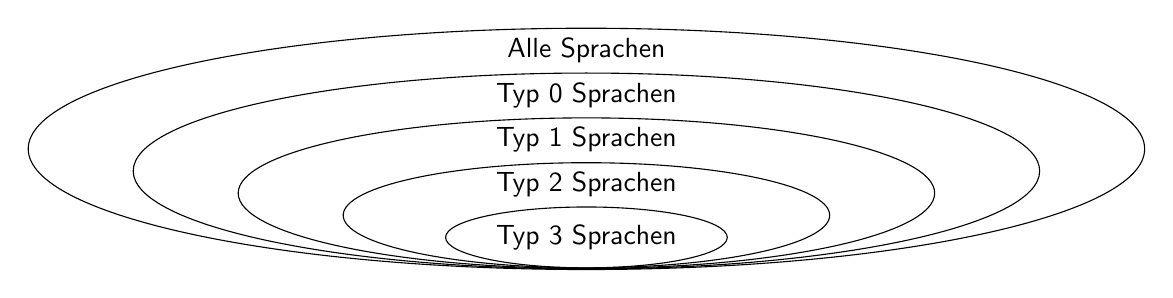
\begin{tikzpicture}[font=\sffamily,breathe dist/.initial=0.01ex]
\foreach \X [count=\Y,remember=\Y as \LastY] in
{Typ 3 Sprachen, Typ 2 Sprachen, Typ 1 Sprachen, Typ 0 Sprachen, Alle Sprachen}
  {\ifnum\Y=1
  \node[ellipse,draw,outer sep=0pt] (F-\Y) {\X};
  \else
  \node[anchor=south] (T-\Y) at (F-\LastY.north) {\X};
  \path let \p1=($([yshift=\pgfkeysvalueof{/tikz/breathe dist}]T-\Y.north)-(F-\LastY.south)$),
  \p2=($(F-1.east)-(F-1.west)$),\p3=($(F-1.north)-(F-1.south)$)
  in ($([yshift=\pgfkeysvalueof{/tikz/breathe dist}]T-\Y.north)!0.5!(F-\LastY.south)$)
  node[minimum height=\y1,minimum width={\y1*\x2/\y3},
  draw,ellipse,inner sep=0pt] (F-\Y){};
  \fi}
\end{tikzpicture}

Eine Sprache $L$ bezeichnen wir als Typ-$n$-Sprache, wenn eine
Typ-$n$-Grammatik G existiert, die $L$ erzeugt. Die Menge aller
Typ-$n$-Sprachen notieren wir mit dem Symbol $\mathcal{L}_1$. Zwischen
den verschiedenen Sprachklassen besteht die folgende
Inklusionsbeziehung:

$\mathcal{L}_0 \supset \mathcal{L}_1 \supset \mathcal{L}_2 \supset \mathcal{L}_3$

%-----------------------------------------------------------------------
%
%-----------------------------------------------------------------------

\noindent
Die Sprache

\begin{itemize}
\item $L_3 = \{(ab)^n \, | \, n \in \mathbb{N}\}$
ist regulär (Typ 3 Sprache)

\item $L_2 = \{a^n b^n \, | \, n \in \mathbb{N}\}$
ist kontextfrei (Typ 2 Sprache), aber nicht regulär

\item $L_1 = \{a^n b^n c^n \, | \, n \in \mathbb{N}\}$
ist kontextsensitiv (Typ 1 Sprache), aber nicht kontextfrei

\item $L_0 = \{a^{(2^n)}\, | \, n \in \mathbb{N}\}$
ist eine Typ 0 Sprache\footcite[Seite 15]{theo:fs:1}
\end{itemize}

%-----------------------------------------------------------------------
%
%-----------------------------------------------------------------------

Ein \memph{Terminalsymbol} (auch Terminalzeichen oder kurz Terminal
genannt) einer formalen Grammatik ist ein Symbol, das einzeln
\memph{nicht weiter durch eine Produktionsregel ersetzt werden
kann}.\footcite{wiki:terminal}

Eine Produktionsregel (auch Regel, Produktion oder Ersetzungsregel
genannt) ist in der Theorie formaler Grammatiken eine Regel, die angibt,
wie \memph{aus Wörtern durch eine Grammatik neue Wörter bzw.
Symbolfolgen produziert} werden.\footcite{wiki:produktionsregel}

%-----------------------------------------------------------------------
%
%-----------------------------------------------------------------------

\section{Grammatik reguläre Sprachen}

\begin{description}
\item[Alphabete]

Die Symbole, aus denen Eingabewörter bestehen können, fassen wir in
einer Menge, dem Eingabealphabet, zusammen. Dabei wollen wir nur
endliche Eingabealphabete zulassen. Ihre Elemente heißen Symbole oder
Buchstaben. Zur Bezeichnung von Eingabealphabeten wird zumeist das
Symbol $\Sigma$ (Sigma) benutzt.
\footcite[Seite 15]{vossen}

\item[Wörter]
Die endlich langen Zeichenfolgen, die über einem Alphabet $\Sigma$
gebildet werden können, heißen Wörter über $\Sigma$. Wörter entstehen,
indem Symbole oder bereits erzeugte Wörter aneinandergereiht
(miteinander verkettet, konkateniert) werden.

$\Sigma^*$ , die Menge aller Wörter, die über dem Alphabet $\Sigma$
gebildet werden kann, ist wie folgt definiert:

\begin{enumerate}
\item Jeder Buchstabe $a \in \Sigma$ ist auch ein Wort über $\Sigma$,
d.\,h. $a \in \Sigma^*$.

\item Werden bereits konstruierte Wörter hintereinandergeschrieben,
entstehen neue Wörter, d.\,h. sind $v, w \in Σ^*$ , dann ist auch ihre
Verkettung (Konkatenation) $v, w \in Σ^*$ .

\item $\epsilon$, das leere Wort, ist ein Wort über (jedem Alphabet)
$\Sigma$, d.\,h. es gilt immer $\epsilon \in Σ^*$. $\epsilon$ ist ein
definiertes Wort ohne „Ausdehnung“. Es hat die Eigenschaft: $\epsilon w
= w \epsilon = w$ für alle $w \in Σ^*$.
\end{enumerate}

Mit $\Sigma^+$ bezeichnen wir die Menge aller Wörter über $\Sigma$ ohne
das leere Wort, d.h. $\Sigma^+ = \Sigma^∗ - \{ \epsilon \}$.
\footcite[Seite 16]{vossen}
\end{description}

Sei $\Sigma$ ein Alphabet. Eine formale Sprache $L$ ist eine Teilmenge
aller Wörter über $\Sigma$:

\begin{displaymath}
L \subseteq \Sigma^*
\end{displaymath}

\bigskip

\noindent
Eine Grammatik ist ein 4-Tupel mit $G = (V, \Sigma, P, S)$ und besteht aus:

\begin{itemize}
\item Einer endlichen Menge $V$ von \memph{Variablen} (Nonterminale)

\item Dem endlichen \memph{Terminalalphabet} $\Sigma$ mit $\Sigma \cap V
= \emptyset$

\item Der endlichen Menge an \memph{Produktionen}

\item Und einer \memph{Startvariablen} $S$ mit $S \in V$
\end{itemize}

%-----------------------------------------------------------------------
%
%-----------------------------------------------------------------------

\section{Reguläre Ausdrücke\footcite[Seite 22]{theo:fs:1}}

Es sind nur die vier Zeichen in „klassischen“ regulären Ausdrücke
erlaubt $*$, $+$, $|$, $()$.

Sprache aller Wörter über \liAlphabet{a,b}
\begin{itemize}
\item $(a | b)^*$, auch das leere Wort
\item $(a | b)^+$, ohne das leere Wort
\item Alle Wörter über \liAlphabet{a,b}, die auf $a$ enden
$(a|b)^*a$
\item Alle Wörter über \liAlphabet{a,b}, die das Teilwort $bb$ enthalten
$(a|b)^*bb(a|b)^*$
\end{itemize}

%----------------------------------------------------------------------
%
%-----------------------------------------------------------------------

\section{Beispiel:}

$G = (V, \Sigma, P, S)$ mit

$V = \{Z, A\}$

\liAlphabet{0, 1}

\begin{liProduktionsRegeln}
Z -> 1a | 1,
A -> 1A | 0A | 1
\end{liProduktionsRegeln}

Eine reguläre Sprache wird durch eine reguläre Grammatik erzeugt, d.\,h.
eine Grammatik mit Produktionsregeln der Form:

$A \rightarrow \epsilon$ oder $A \rightarrow 1$ oder $A \rightarrow 0A$

linke Seite: ein Nonterminal rechte Seite: $\epsilon$ oder ein Terminal
oder ein Terminal gefolgt von einem Nonterminal

Man spricht hierbei auch von rechtslinearer Grammatik (es gibt auch
linkslineare Grammatiken)

$G = (\{Z, A\}, \{0, 1\}, P, Z)$

Syntaxbaum zu 100101
\begin{center}
\begin{tikzpicture}[level distance=0.7cm]
\Tree [.Z
  [.1 ] [.A
    [.0 ] [.A
      [.0 ] [.A
        [.1 ] [.A
          [.0 ] [.A
            [.1 ]
          ]
        ]
      ]
    ]
  ]
]
\end{tikzpicture}
\end{center}

%-----------------------------------------------------------------------
%
%-----------------------------------------------------------------------

\section{Deterministische endliche Automaten}

Ein deterministischer endlicher Automat (\memph{DEA}; englisch
deterministic finite state machine oder deterministic finite automaton,
\memph{DFA}) ist ein endlicher Automat, der unter \memph{Eingabe eines
Zeichens} seines Eingabealphabetes (den möglichen Eingaben) von einem
Zustand, in dem er sich befindet, in einen \memph{eindeutig bestimmten
Folgezustand} wechselt.
\footcite{wiki:dea}

Einen endlichen Automaten können wir uns als eine „Black Box“
vorstellen, in die wir etwas eingeben können und die sich aufgrund einer
Folge von Eingaben in einem entsprechenden Zustand befindet. In
Abhängigkeit von ihrem jeweiligen Zustand und einer erfolgten Eingabe
geht sie in einen Folgezustand über. Befindet sich die Black Box nach
der Abarbeitung der Eingabefolge in einem ausgezeichneten Zustand, einem
so genannten Endzustand, dann handelt es sich um eine von ihr
akzeptierte Folge, falls sie sich nicht in einem Endzustand befindet,
hat sie die Eingabe nicht akzeptiert.
\footcite[Seite 11]{vossen}

Automaten sind \memph{deterministisch}, wenn es in jedem Zustand für jedes
Eingabesymbol \memph{höchstens einen Folgezustand} gibt.
\footcite[Seite 28]{vossen}

Ein DEA/DFA ist ein 5-Tupel ($Z, \Sigma, \delta, E, z_0$) mit

\begin{description}
\item[$Z$:] Menge der Zustände (endlich)
\item[$\Sigma$:] Eingabealphabet mit (endlich)
\item[$\delta$:] $Z \times \Sigma \rightarrow Z$ Zustandsübergangsfunktion
\item[$E$:] Menge der Endzustände
\item[$z_0$:] Startzustand\footcite[Seite 26]{theo:fs:1}
\end{description}

%-----------------------------------------------------------------------
%
%-----------------------------------------------------------------------

\section{Pumping Lemma}

https://studyflix.de/informatik/pumping-lemma-1445

Pumping-Lemma für reguläre Sprachen:

Sei $L$ eine reguläre Sprache. Dann gibt es eine Zahl $j$, sodass für
alle Wörter $ω ∈ L$ mit $|\omega| \geq j$ jeweils eine Zerlegung $\omega
= uvw$ existiert, sodass die folgenden Eigenschaften erfüllt sind:

\begin{enumerate}
\item $|v| \geq 1$
\item $|uv| \leq j$
\item Für alle $i = 0, 1, 2, \dots$ gilt $uv^iw \in L$
\end{enumerate}

Das Pumping-Lemma wird verwendet, um zu zeigen, dass eine
Sprache nicht regulär ist (Widerspruchsbeweis).

%%
%
%%

\subsection{Beispiel}

$L = \{a^n b^n | n \in \mathbb{N})$

Ich behaupte, $L$ sei regulär.

\begin{enumerate}
\item Also gibt es eine Pumpzahl. Sie sei j.
\item (Wähle geschickt ein „langes“ Wort...)
$a^j b^j$ ist ein Wort aus $L$, das sicher langer als $j$ ist.
\item Da $L$ regulär ist, muss es nach dem Pumping-Lemma auch für dieses
Wort eine Zerlegung geben:
\end{enumerate}

$a^j b^j = uvw$ mit $|v| \geq 1$ und $|uv| \leq j$

Weil $uv$ höchstens $j$ lang ist, kann es im Fall von $a^j b^j$ nur aus
$a$‘s bestehen. Da $v$ mindestens ein Zeichen enthält, ist das
mindestens ein $a$. Pumpen führt nun zu mehr $a$‘s als $b$‘s und also zu
einem Wort, das nicht in der Sprache ist. (Widerspruch!)\footcite{wiki:pumping}

$\Rightarrow$ Die Behauptung war falsch!
$\Rightarrow$ $L$ ist nicht regulär!
\footcite[Seite 63-64]{theo:fs:1}

%-----------------------------------------------------------------------
%
%-----------------------------------------------------------------------

\section{Minimierungsalgorithmus\footcite[Seite 47-57]{vossen}}

\footcite[Seite 51-62]{theo:fs:1}

https://studyflix.de/informatik/dea-minimieren-1212

%-----------------------------------------------------------------------
%
%-----------------------------------------------------------------------

\section{Äquivalenzklassen (nach Myhill, Nerode)\footcite{theo:fs:}}

Zwei Wörter $x, y \in \Sigma^*$ sind äquivalent bzgl. einer Sprache $L$,
wenn für alle $z \in Σ^*$ gilt:

$xz \in L <=> yz \in L$

Eine Sprache $L$ ist genau dann regulär, wenn sie endlich viele
Äquivalenzklassen erzeugt.

Die Anzahl der Äquivalenzklassen einer Sprache entspricht der
minimalen Anzahl von Zustanden eines DEA, der diese Sprache
erkennt. (Darauf fußt der Minimalisierungsalgorithmus.)

\subsection{Beispiel zu Äquivalenzklassen}

$(1|11|111)0^*$ sind alle Binärzahlen, die mit einer, zwei oder drei
Einsen beginnen, gefolgt von beliebig vielen Nullen.

\begin{enumerate}
\item Sind x=1 und y=10 in der selben Äquivalenzklasse?

Nein, denn anfügen von $z=1$:

\begin{itemize}
\item $xz = 11$ erlaubtes Wort

\item $yz = 101$ unerlaubtes Wort
\end{itemize}

\item Sind $x=1$ und $y=11$ in der selben Äquivalenzklasse?

Nein, denn anfügen von $z=11$:

\begin{itemize}
\item $xz = 111$ erlaubtes Wort
\item $yz = 1111$ unerlaubtes Wort
\end{itemize}

\item Sind $x=10$ und $y=110$ in der selben Äquivalenzklasse?

Ja, fügt man nur 0en an, sind die Wörter in $L$, fügt man auch 1en an,
sind sie nicht in $L$.
\end{enumerate}

\subsection{Äquivalente Zustände}

Zwei Zustande $z$, $z'$ eines deterministischen Automaten sind
äquivalent, wenn für alle möglichen Eingaben der Automat entweder in
beiden Fallen in einen (nicht notwendig gleichen) Endzustand oder in
beiden Fallen in einen (nicht notwendig gleichen) Nicht-Endzustand
übergeht.

Äquivalente Zustände können zu einem Zustand verschmolzen
werden.

%-----------------------------------------------------------------------
%
%-----------------------------------------------------------------------

\section{Nichtdeterministische endliche Automaten}

Ein nichtdeterministischer endlicher Automat (NEA; englisch
nondeterministic finite automaton, NFA) ist ein endlicher Automat, bei
dem es für den \memph{Zustandsübergang mehrere gleichwertige
Möglichkeiten} gibt. Im Unterschied zum deterministischen endlichen
Automaten sind die Möglichkeiten nicht eindeutig, dem Automaten ist also
nicht vorgegeben, welchen Übergang er zu wählen hat.\footcite{wiki:nea}

\begin{center}
\begin{tikzpicture}[->]
\node[state,initial] (p) {p};
\node[state,accepting,right=of p] (q) {q};

\path (p) edge[above] node{1} (q);

\path (p) edge[loop,above] node{0,1} (q);
\end{tikzpicture}
\end{center}

Nichtdeterministische endliche Automaten sind Automaten, in denen es zu
einem Zustand und einem Eingabesymbol mehrere Folgezustände geben kann.
\footcite[Seite 28]{vossen}

Ein NEA/NFA ist ein 5-Tupel ($Z, \Sigma, \sigma, E, z_0$) mit

\begin{description}
\item[$Z$:] Menge der Zustände (endlich)
\item[$\Sigma$:] Eingabealphabet mit (endlich)
\item[$\delta$:] $Z \times \Sigma \rightarrow 2^Z$ Zustandsübergangsfunktion
\item[$E$:] Menge der Endzustände
\item[$z_0$:] Startzustand\footcite[Seite 30]{theo:fs:1}
\end{description}

Potenzmenge\footcite{wiki:potenzmenge}

\let\p=\liPotenzmengeOhneMathe

Beispiel: $Z = \p{ z_1, z_2 }$

$2^Z = \{\p{}, \p{z_1 }, \p{z_2 }, \p{z_1 , z_2 }\}$

%-----------------------------------------------------------------------
%
%-----------------------------------------------------------------------

\section{Potenzmengenalgorithmus NEA $\rightarrow$ DEA\footcite[Seite 35-48]{theo:fs:1}}

\begin{itemize}
\item Starte im Anfangszustand (in der Menge der Anfangszustände).

\item Gib für jedes Zeichen die Menge der erreichbaren Zustände an.

\item Wiederhole diesen Schritt für jede neu erreichte Menge an
Zuständen.

\item Die Zustandsmengen sind die Zustände des DEA.

\item Mengen, die „alte“ Endzustände enthalten, sind Endzustände des
neuen DEA.\footcite{wiki:potenzmengenkonstruktion}
\end{itemize}
\literatur

\end{document}
